\begin{figure}
    \begin{center}
    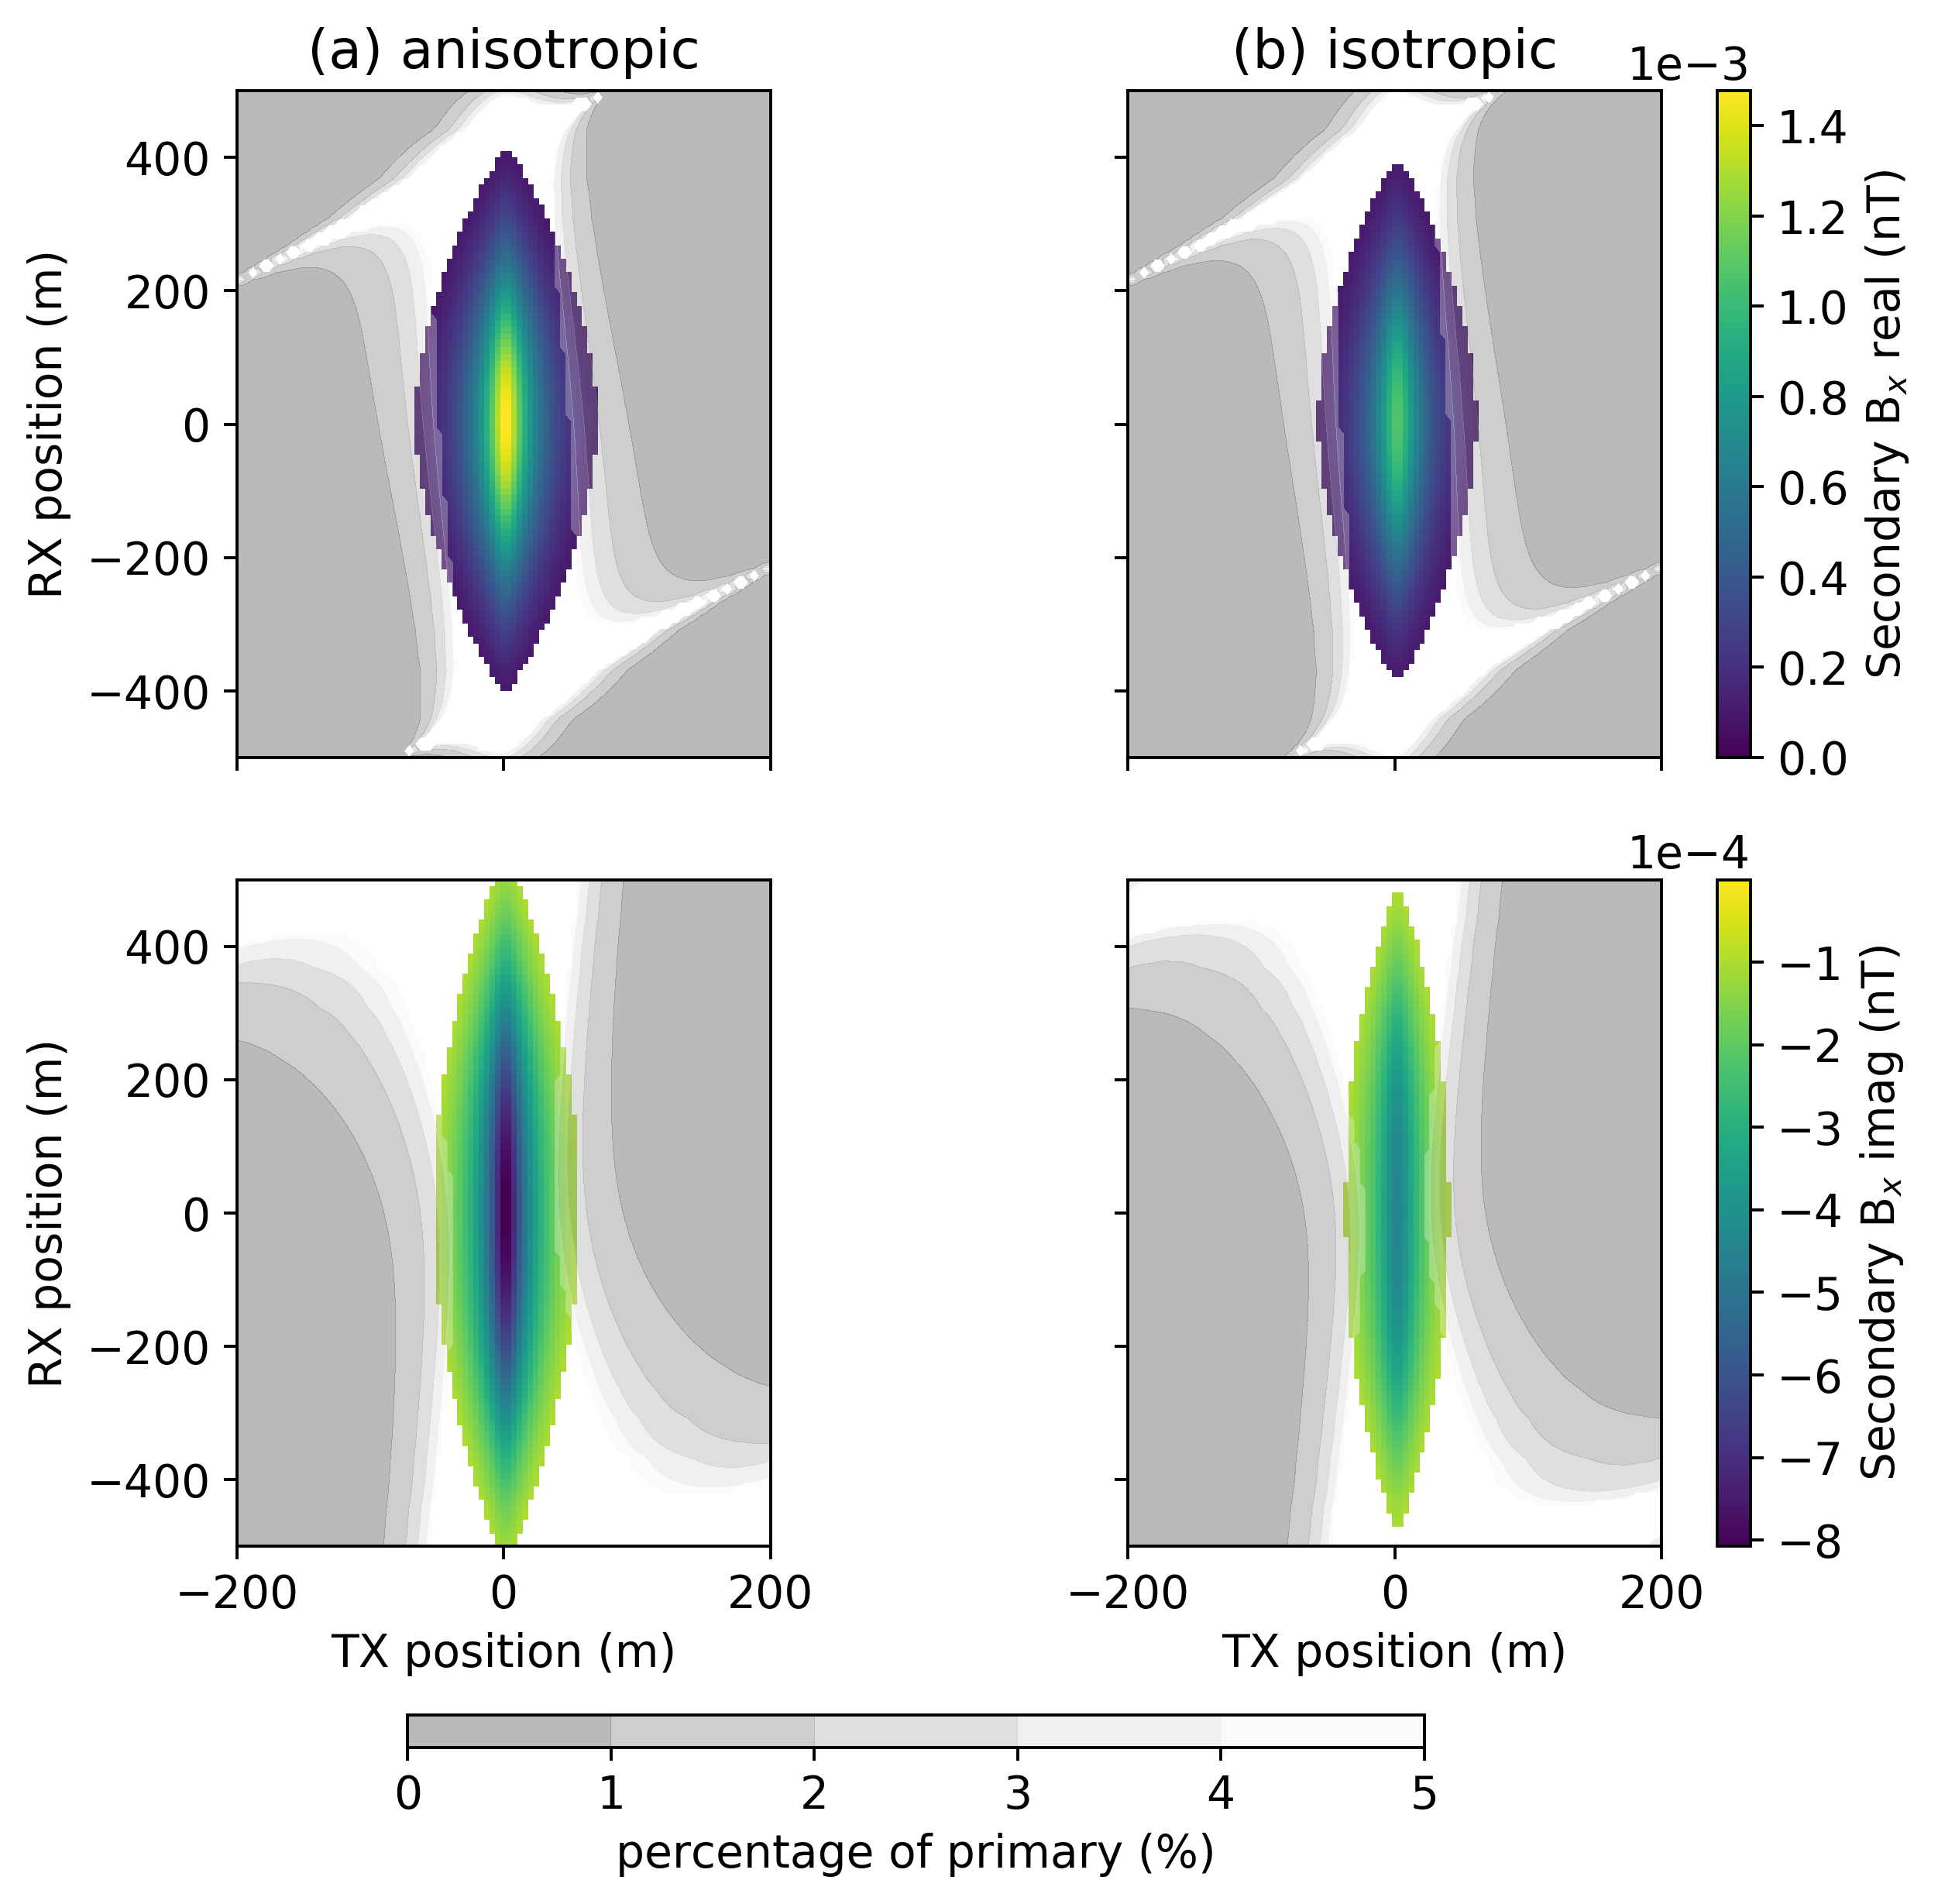
\includegraphics[width=\textwidth]{figures/phys_prop_model/crosswell_data100.png}
    \end{center}
\caption{
    Simulated secondary magnetic field data for: (a) the anisotropic fracture model and
    (b) the isotropic fracture model, in a crosswell survey conducted at 100Hz.
    The top row shows the real component and the bottom row shows
    the imaginary component of the measured magnetic flux (nT).
    In all plots, the x-axis shows the transmitter location relative to the center
    of the fracture, the y-axis shows the receiver location, and the color indicates the secondary
    magnetic flux with respect to a 0.1 S/m whole-space. Values beneath the noise floor of $10^{-4}$ nT
    have been masked and display as white. To display the signal as a percentage of the primary, we have
    included a semi-transparent overlay between 0\% and 5\%; low percentage values plot as darker
    greys.
}
\label{fig:crosswell_data100}
\end{figure}
